% ------------------------------------------------------------------------------
% TYPO3 CMS 6.2 LTS - What's New - Chapter "Install Tool" (Dutch Version)
%
% @author	Christiaan Wiesenekker <cwiesenekker@gmail.com>
% @author	Ric van Westhreenen <ric.vanwesthreenen@typo3.org>
% @license	Creative Commons BY-NC-SA 3.0
% @link		http://typo3.org/download/release-notes/whats-new/
% @language	Dutch
% ------------------------------------------------------------------------------
% Chapter: Install Tool
% ------------------------------------------------------------------------------

\section{Install Tool}
\begin{frame}[fragile]
	\frametitle{Install Tool}

	\begin{center}\huge{Hoofdstuk 1:}\end{center}
	\begin{center}\huge{\color{typo3darkgrey}\textbf{De Install Tool}}\end{center}

\end{frame}

% ------------------------------------------------------------------------------
% Installation
% ------------------------------------------------------------------------------

\begin{frame}[fragile]
	\frametitle{Install Tool}
	\framesubtitle{Installatie}

	\begin{itemize}
		\item Slechts \underline{een} package is nodig voor een installatie:\newline
				\texttt{typo3\_src-6.2.x.tar.gz} (bestandsgrootte: ong. 20MB)
		\item "Dummy" en "Blank" packages zijn voortaan overbodig
		\item Installatie:
			\begin{itemize}
				\item Pak de bron package uit in de web root directory
				\item Ga met de webbrowser naar de web root
				\item TYPO3 Installer start 1-2-3-4-staps wizard
			\end{itemize}

	\end{itemize}

\end{frame}

% ------------------------------------------------------------------------------
% Installation
% ------------------------------------------------------------------------------

\begin{frame}[fragile]
	% \TabPositions{2cm}

	\frametitle{Install Tool}
	\framesubtitle{Installatie}

	\begin{itemize}
		\item De Installer zorgt ervoor dat alle benodigde bestanden en directories op de juiste plaats staan
		\item Bestanden nodig voor een specifieke setup worden automatisch gemaakt
		\item De volgende symbolische links \underline{moeten} aanwezig zijn:

		\begin{itemize}
			\item \texttt{typo3\_src}	\tabto{2cm} (verwijst naar de TYPO3 bron directory)
			\item \texttt{typo3}		\tabto{2cm} (verwijst naar de directory: \texttt{typo3\_src/typo3})
			\item \texttt{index.php}	\tabto{2cm} (verwijst naar het bestand: \texttt{typo3\_src/index.php})
		\end{itemize}

		\item Geen andere bestanden/directories zijn verder nodig voor de installatie van TYPO3!
		\item Directory \texttt{t3lib} is verwijderd
		\item Nadere details: TYPO3 Installation and Upgrade Guide\newline
			\url{http://docs.typo3.org/typo3cms/InstallationGuide}

	\end{itemize}

\end{frame}

% ------------------------------------------------------------------------------
% Re-Development
% ------------------------------------------------------------------------------

\begin{frame}[fragile]
	\frametitle{Install Tool}
	\framesubtitle{Her-ontwikkeld}

	\begin{columns}[T]

		\begin{column}{.5\textwidth}
			\begin{itemize}
				\item Her-ontwikkeld vanaf scratch in Fluid
				\item \underline{Eerste} stap test de systeem omgeving en koppelt problemen terug
				\item Teruggekoppelde problemen kunnen worden opgelost\newline (en opnieuw getest) of je kunt ze negeren
				\item Verkeerde core setup (bijvoorbeeld geen gebruik van symbolic links) wordt ook gezien als een probleem
			\end{itemize}
		\end{column}

		\begin{column}{.5\textwidth}
			\begin{figure}\vspace*{-0.4cm}
				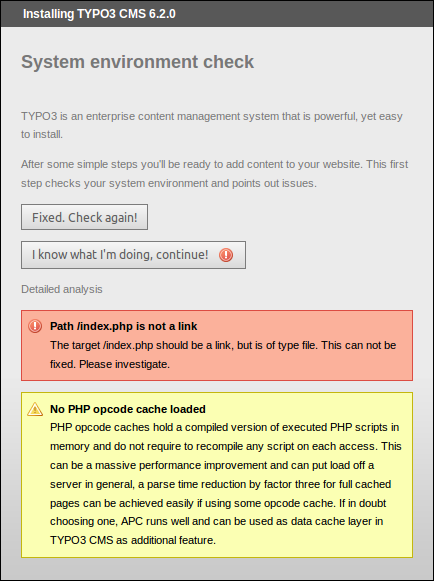
\includegraphics[width=0.8\linewidth,height=5cm]{Images/InstallTool/SystemEnvironmentCheck.png}
			\end{figure}
		\end{column}

	\end{columns}

\end{frame}

% ------------------------------------------------------------------------------
% Re-Development
% ------------------------------------------------------------------------------

\begin{frame}[fragile]
	\frametitle{Install Tool}
	\framesubtitle{Her-ontwikkeld}

	\begin{columns}[T]

		\begin{column}{.5\textwidth}
			\begin{itemize}
				\item \underline De {tweede} stap geeft gebruikers de mogelijkheid om de database gegevens toe te voegen
				\item De verschillende koppelingen zijn te selecteren
					\begin{itemize}
						\item TCP/IP gebaseerde koppeling
						\item Socket gebaseerde koppeling
					\end{itemize}
				\item MySQL alternatieven zijn ook mogelijk
			\end{itemize}
		\end{column}

		\begin{column}{.5\textwidth}
			\begin{figure}\vspace*{-0.4cm}
				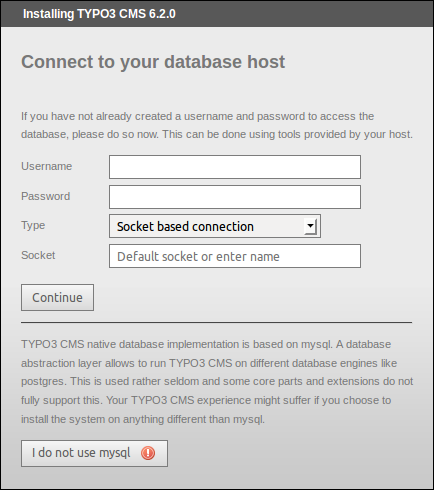
\includegraphics[width=0.6\linewidth]{Images/InstallTool/DatabaseConnectionDetails.png}
	%			\includegraphics[width=0.8\linewidth,height=5cm]{Images/Dummy_800x800.png}
			\end{figure}
		\end{column}

	\end{columns}

\end{frame}

% ------------------------------------------------------------------------------
% Re-Development
% ------------------------------------------------------------------------------

\begin{frame}[fragile]
	\frametitle{Install Tool}
	\framesubtitle{Her-ontwikkeling}

	\begin{columns}[T]

		\begin{column}{.5\textwidth}
			\begin{itemize}
				\item \underline De {derde} stap biedt gebruikers de mogelijkheid om een database te kiezen of selecteren\newline
					(net als bij TYPO3 < 6.2)
				\item \underline De {vierde} stap biedt gebruikers de mogelijkheid om een password te kiezen voor de "admin" gebruiker\newline (dat is tevens het initiële Install Tool password) en de website naam
			\end{itemize}
		\end{column}

		\begin{column}{.5\textwidth}
			\begin{figure}\vspace*{-0.4cm}
		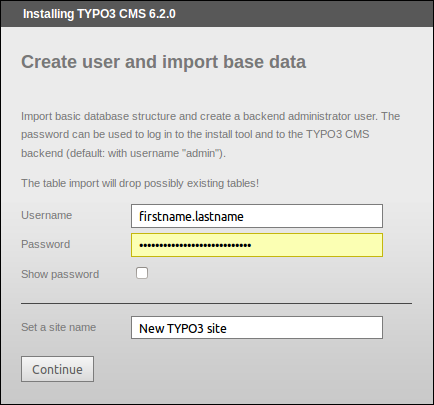
\includegraphics[width=0.6\linewidth]{Images/InstallTool/AdminPasswordAndSiteName.png}
		%		\includegraphics[width=0.8\linewidth,height=5cm]{Images/Dummy_800x800.png}
			\end{figure}
		\end{column}

	\end{columns}

\end{frame}

% ------------------------------------------------------------------------------
% Delete All Cache
% ------------------------------------------------------------------------------

\begin{frame}[fragile]
	\frametitle{Install Tool}
	\framesubtitle{Wis alle cache}

	\begin{itemize}
		\item Nieuwe functie onder "Important actions" dat gebruikers de volledige cache laat wissen
		\item Dit is ook mogelijk als de cache foutieve PHP code bevat\newline
			(dat wellicht een probleem veroorzaakt in TYPO3 CMS)
		\item Passeer een niet-werkende TYPO3 instantie door de install tool rechtstreeks aan te roepen: \texttt{http://example.com/typo3/install}
	\end{itemize}

	\begin{columns}[T]
		\begin{column}{.4\textwidth}
			\begin{figure}\vspace*{-0.4cm}
				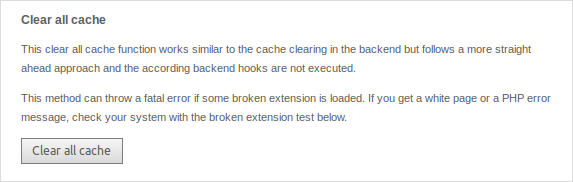
\includegraphics[width=0.6\linewidth]{Images/InstallTool/ClearAllCache.png}
%				\includegraphics[width=0.8\linewidth,height=3cm]{Images/Dummy_800x800.png}
			\end{figure}
		\end{column}
		\begin{column}{.6\textwidth}
			\begin{figure}
				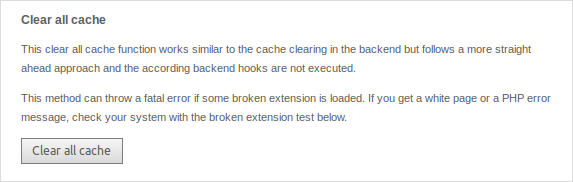
\includegraphics[width=0.6\linewidth]{Images/InstallTool/ClearAllCache.png}
%				\includegraphics[width=0.8\linewidth,height=2.6cm]{Images/Dummy_800x800.png}
			\end{figure}
		\end{column}
	\end{columns}

\end{frame}

% ------------------------------------------------------------------------------
% Delete All Cache
% ------------------------------------------------------------------------------

\begin{frame}[fragile]
	\frametitle{Install Tool}
	\framesubtitle{Wis alle Cache}

	Volgorde van alle acties zodra gekozen is voor "Delete all cache":

	\begin{enumerate}
		\item Inhoud van de directory \texttt{typo3temp/Cache} is verwijderd
		\item Database tabellen \texttt{cf\_*} zijn geleegd
		\item Bestanden \texttt{ext\_localconf.php} en \texttt{ext\_tables.php}\newline
			van extensies worden geladen
		\item \texttt{flushCaches()} wordt uitgevoerd
	\end{enumerate}

\end{frame}

% ------------------------------------------------------------------------------
% Check For Broken Extensions
% ------------------------------------------------------------------------------

\begin{frame}[fragile]
	\frametitle{Install Tool}
	\framesubtitle{Controle op defecte extensies}

	\begin{itemize}
		\item Nieuwe functie onder "Important actions" biedt gebruikers een controle,\newline
			of extensies geladen kunnen worden zonder dat er een probleem optreedt
		\item Erg handig bij een update van TYPO3 4.5 naar 6.2
	\end{itemize}

	\begin{columns}[T]
		\begin{column}{.3\textwidth}
			\begin{figure}\vspace*{-0.4cm}
				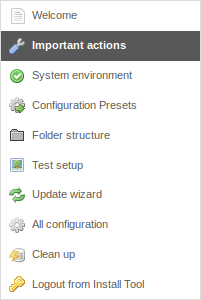
\includegraphics[width=0.7\linewidth]{Images/InstallTool/ImportantActions.png}
			\end{figure}
		\end{column}
		\begin{column}{.7\textwidth}
			\begin{figure}\vspace*{-0.4cm}
				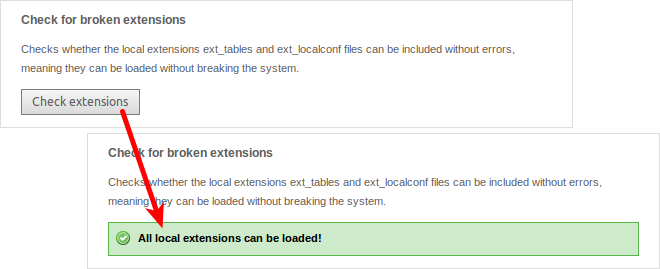
\includegraphics[width=1\linewidth]{Images/InstallTool/CheckForBrokenExtensions.png}
			\end{figure}
		\end{column}
	\end{columns}
\end{frame}

% ------------------------------------------------------------------------------
% Increased Security: Salted Passwords
% ------------------------------------------------------------------------------

\begin{frame}[fragile]
	\frametitle{Install Tool}
	\framesubtitle{Salted Passwords}

	\begin{itemize}
		\item Wanneer een nieuwe backend administrator aangemaakt wordt via de Install Tool, \newline
			maken we gebruik van een \textbf{salted} password\newline
			(hiervoor dient de EXT:saltedpasswords geïnstalleerd, geladen en geconfigureerd te zijn)
		\item De Install Tool password is sowieso een \textbf{salted} password\newline
			(bestaande MD5 hashes worden bij de eerste login automatisch geconverteerd)
	\end{itemize}

	\begin{columns}[T]
		\begin{column}{.3\textwidth}
			\begin{figure}\vspace*{-0.4cm}
				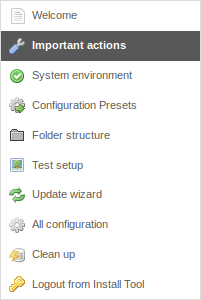
\includegraphics[width=0.7\linewidth]{Images/InstallTool/ImportantActions.png}
			\end{figure}
		\end{column}
		\begin{column}{.7\textwidth}
			\begin{figure}\vspace*{-0.4cm}
				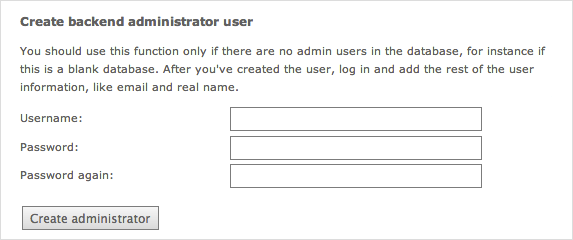
\includegraphics[width=0.9\linewidth]{Images/InstallTool/SaltedPasswords.png}
			\end{figure}
		\end{column}
	\end{columns}

\end{frame}

% ------------------------------------------------------------------------------
% Application Context
% ------------------------------------------------------------------------------

\begin{frame}[fragile]
	\frametitle{Install Tool}
	\framesubtitle{Applicatie Context (1)}

	\begin{itemize}
		\item TYPO3 >= 6.2 neemt de \textbf{Applicatie Context} mee\newline
			\smaller(zoals bekend van TYPO3 Flow)\normalsize
		\item Omgevingsvariabele \texttt{TYPO3\_CONTEXT} bepaalt de context\newline
			\smaller(standaardwaarde: \texttt{Productie}, sub-context als \texttt{Productie/Staging} mogelijk)\normalsize

			\begin{lstlisting}
				# Bestand: .htaccess
				# Regels om de Applicatie Context in te richten op basis van de hostname:

				RewriteCond %{HTTP_HOST} ^dev\.example\.com$
				RewriteRule (.*) $1 [E=TYPO3_CONTEXT:Development]

				RewriteCond %{HTTP_HOST} ^www\.example\.com$
				RewriteRule (.*) $1 [E=TYPO3_CONTEXT:Production]

				# Sets an environment variable, which is then available to TYPO3 CMS:
				SetEnv TYPO3_CONTEXT Production
			\end{lstlisting}

	\end{itemize}

\end{frame}

% ------------------------------------------------------------------------------
% Application Context
% ------------------------------------------------------------------------------

\begin{frame}[fragile]
	\frametitle{Install Tool}
	\framesubtitle{Vooraf ingestelde TYPO3\_CONF\_VAR instellingen}

	\begin{columns}[T]
		\begin{column}{.5\textwidth}

			\begin{itemize}
				\item Bepaalde TYPO3\_CONF\_VAR instellingen kunnen worden ingesteld in de Install Tool
				\item Controls presets als debug output, deprecation log, devIPmask en andere systeem logs en log levels
				\item Ingebouwde contexts: "Productie" en "Development"\newline
					(custom configuratie is ook mogelijk)
			\end{itemize}

		\end{column}
		\begin{column}{.5\textwidth}

			\begin{figure}\vspace*{-0.4cm}
				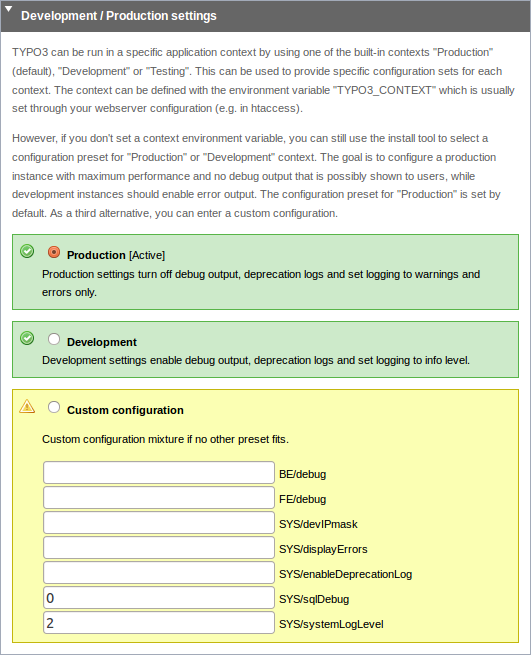
\includegraphics[width=5cm,height=5cm]{Images/InstallTool/ApplicationContext.png}
			\end{figure}

		\end{column}
	\end{columns}

\end{frame}

% ------------------------------------------------------------------------------
% Improved Usability
% ------------------------------------------------------------------------------

\begin{frame}[fragile]
	\frametitle{Install Tool}
	\framesubtitle{Verbeterde Usability}

	\begin{columns}[T]
		\begin{column}{.5\textwidth}

			\begin{itemize}
				\item Plaatsing van het linkermenu als je scrolled is verbeterd
				\item Plaatsing van de knop "Write configuration" is naar de onderkant verplaatst
				\item Invoer bij "All Configuration" is gegroepeerd (een sectie klapt uit bij een muisklik op een kopje) en sorteerbaar
			\end{itemize}

		\end{column}
		\begin{column}{.5\textwidth}

			\begin{figure}\vspace*{-0.4cm}
				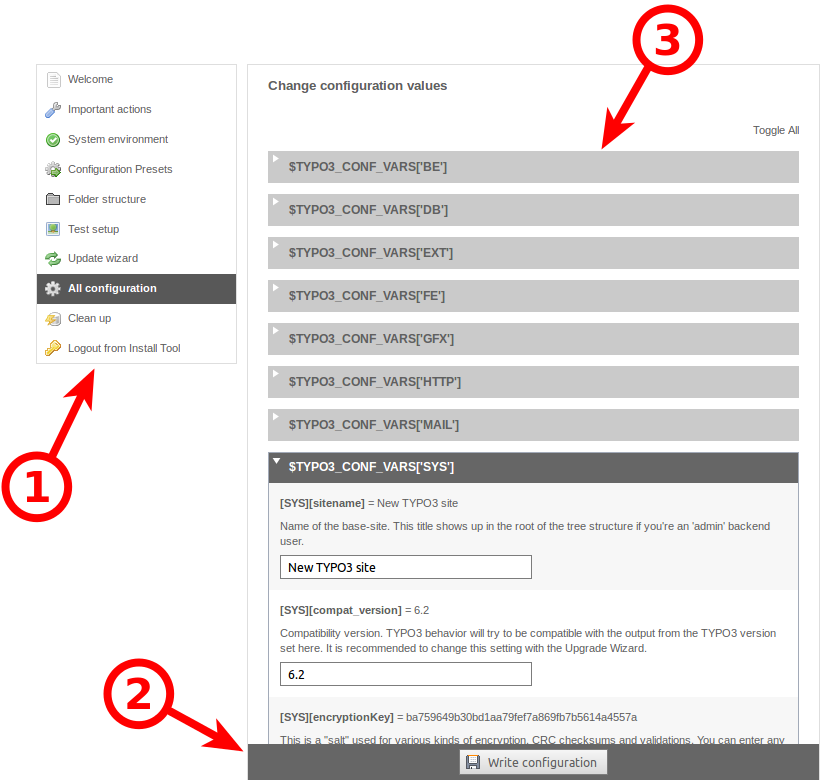
\includegraphics[width=5cm,height=5cm]{Images/InstallTool/ImprovedUsability.png}
			\end{figure}

		\end{column}
	\end{columns}

\end{frame}

% ------------------------------------------------------------------------------
% Human-Friendly Error Codes
% ------------------------------------------------------------------------------

\begin{frame}[fragile]
	\frametitle{Install Tool}
	\framesubtitle{Leesbare Error Codes}

	\begin{itemize}
		\item Zinvolle trefwoorden kunnen worden gebruit voor de volgende opties:\newline
			(TYPO3 < 6.2: alleen nummerieke waardes)
	\end{itemize}

	\begin{columns}[T]
		\begin{column}{.5\textwidth}
			\advance\leftskip+0.8cm

			\smaller
				\texttt{[SYS][errorHandlerErrors]}\newline
				\texttt{[SYS][exceptionalErrors]}\newline
				\texttt{[SYS][syslogErrorReporting]}\newline
				\texttt{[SYS][belogErrorReporting]}\newline
			\normalsize

		\end{column}
		\begin{column}{.5\textwidth}

			\begin{figure}\vspace*{-0.4cm}
				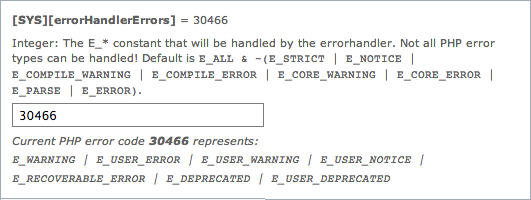
\includegraphics[width=5cm,height=3cm]{Images/InstallTool/HumanFriendlyErrorCodes.png}
			\end{figure}

		\end{column}
	\end{columns}

	\begin{itemize}
		\item Een Extbase ViewHelper \textbf{format.phpErrorCode} zorgt voor de vertaalslag naar PHP error codes
	\end{itemize}

	% *TODO* image/illustration with E_ALL, E_ERROR, etc.?

\end{frame}

% ------------------------------------------------------------------------------
% Errors In Folder Structure
% ------------------------------------------------------------------------------

\begin{frame}[fragile]
	\frametitle{Install Tool}
	\framesubtitle{Errors In Folder Structuur}

	\begin{itemize}
		\item Errors in de "Folder Structuur" worden getoond via een badge (omcirkelt nummer)
	\end{itemize}

	\begin{figure}
		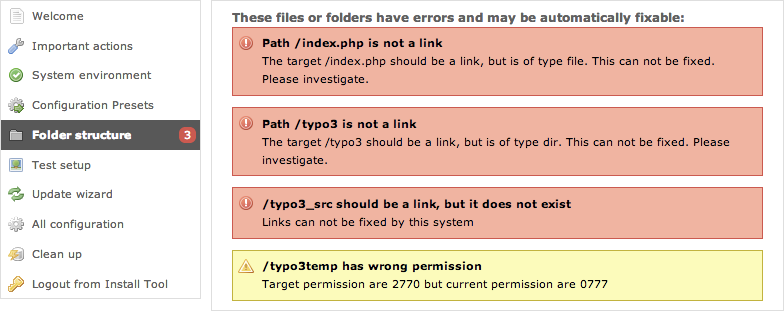
\includegraphics[width=0.95\linewidth]{Images/InstallTool/ErrorsInFolderStructure.png}
	\end{figure}

\end{frame}

% ------------------------------------------------------------------------------
% Core Updates
% ------------------------------------------------------------------------------

\begin{frame}[fragile]
	\frametitle{Install Tool}
	\framesubtitle{Core Updates}

	\begin{itemize}
		\item Update van de TYPO3 core naar de laatste minor versie kan met een klik op de knop
		\item Environment variabelen \texttt{TYPO3\_DISABLE\_CORE\_UPDATER=1} zet deze optie uit
	\end{itemize}

	\begin{figure}
		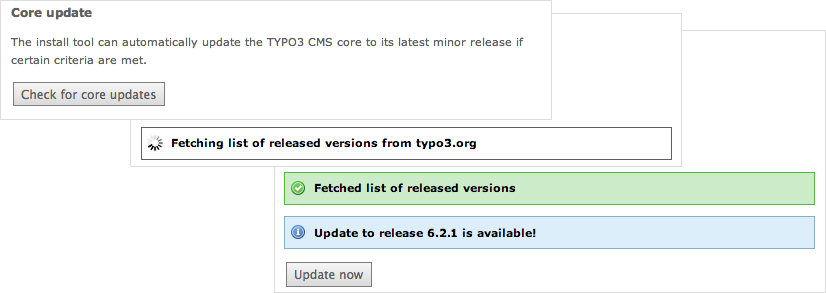
\includegraphics[width=0.95\linewidth]{Images/InstallTool/CoreUpdate.png}
	\end{figure}

\end{frame}

% ------------------------------------------------------------------------------
% Miscellaneous
% ------------------------------------------------------------------------------

\begin{frame}[fragile]
	\frametitle{Install Tool}
	\framesubtitle{Overige}

	\begin{itemize}
		\item Alle formulieren zijn beschermd tegen CSRF (\textit{cross-site request forgery}) 		\item De Install Tool gebruikt een vereenvoudigde Fluid Standalone View
		\item Alleen essentiele TYPO3 functies worden geladen\newline
			(Corrupte \texttt{ext\_localconf.php} of \texttt{ext\_tables.php} van extensies kunnen de Install Tool niet meer kapotmaken)
		\item Nieuw start punt:	\tabto{3.2cm} \texttt{typo3/sysext/install/Start/Install.php}\newline
			Voorheen:					\tabto{3.2cm} \texttt{typo3/install/index.php}\newline
									\tabto{3.2cm} (redirect van oud naar nieuw is aanwezig)
		\item Cache is uitgezet, zodat de Install Tool blijft werken, ook als de cache foutieve PHP code bevat
	\end{itemize}

\end{frame}

% ------------------------------------------------------------------------------
% Miscellaneous
% ------------------------------------------------------------------------------

\begin{frame}[fragile]
	\frametitle{Install Tool}
	\framesubtitle{Overige}

	\begin{itemize}
		\item Controleer of de PHP optie \texttt{xdebug.max\_nesting\_level} een waarde van 250 of hoger toont (de standaardwaarde van "100" kan problemen veroorzaken)
		\item "Relaxed permission check":

			\small
				Als de web root folder niet de juiste rechten kent (bv. "2770"),
				en dit niet aangepast kan worden, omdat de foldereigenaar anders is dan de gebruiker die de Install Tool draait, dan zal de eerste stap van het installatieproces worden afgebroken.
					De optie "targetPermissionRelaxed" omzeilt dit probleem als de permissies niet ideaal zijn waardoor de installatie verder kan worden doorgezet zolang de noodzakelijke subfolders aangemaakt kunnen worden.
			\normalsize

		% *TODO* wait until further details are available
		% \item (German) Es wurde ein „Distribution management“ zugefügt (um Distributionen wie „Introduction Package“ oder „Government Package“ während der Installation zu laden und zu konfigurieren)

		% *TODO* double check, when beta2 has been released
		% \item phpinfo() has been removed from Install Tool

	\end{itemize}

\end{frame}

% ------------------------------------------------------------------------------
% Miscellaneous
% ------------------------------------------------------------------------------

\begin{frame}[fragile]
	\frametitle{Install Tool}
	\framesubtitle{Overige}

	\begin{itemize}
		\item De optie (keys) is verwijderd uit de Install Tool\newline
			(en daarom ook uit het bestand \texttt{LocalConfiguration.php}):
	\end{itemize}

	\begin{columns}[T]
		\begin{column}{.5\textwidth}
			\advance\leftskip+0.8cm
			\smaller
				\texttt{BE/loginLabels}\newline
				\texttt{BE/loginNews}\newline
				\texttt{BE/useOnContextMenuHandler}\newline
				\texttt{EXT/em\_mirrorListURL}\newline
				\texttt{EXT/em\_wsdlURL}\newline
				\texttt{EXT/extList}\newline
				\texttt{EXT/extList\_FE}\newline
				\texttt{EXT/noEdit}\newline
			\normalsize
		\end{column}
		\begin{column}{.5\textwidth}
			\smaller
				\texttt{FE/defaultTypoScript\_editorcfg}\newline
				\texttt{FE/simulateStaticDocuments}\newline
				\texttt{GFX/noIconProc}\newline
				\texttt{GFX/TTFLocaleConv}\newline
				\texttt{SYS/additionalAllowedClassPrefixes}\newline
				\texttt{SYS/caching/cacheBackends}\newline
				\texttt{SYS/caching/cacheFrontends}\newline
				\texttt{SYS/extCache}\newline
				\texttt{SYS/T3instID}\newline
			\normalsize
		\end{column}

	\end{columns}

\end{frame}

% ------------------------------------------------------------------------------

